\documentclass[a4paper,10pt,twoside]{article}
\usepackage[polish]{babel}
\usepackage[utf8]{inputenc}
\usepackage[T1]{fontenc}
\usepackage{indentfirst}
\usepackage[top=2.5cm, bottom=2.5cm, left=2.5cm, right=2.5cm]{geometry}
\usepackage{graphicx}
\usepackage{amsmath}
\usepackage{booktabs}

\begin{document}

\newcommand{\unit}[1]{\thinspace \mathrm{#1}}

\begin{center}
\bgroup
\def\arraystretch{1.5}
\begin{tabular}{|c|c|c|c|c|c|}
	\hline
	EAIiIB & \multicolumn{2}{|c|}{Piotr Morawiecki, Tymoteusz Paszun} & Rok II & {Grupa 3a} & {Zespół 6} \\
	\hline
	\multicolumn{3}{|c|}{\begin{tabular}{c}Temat: Wahadła fizyczne \end{tabular}} & 
	\multicolumn{3}{|c|}{\begin{tabular}{c}Numer ćwiczenia: 1 \end{tabular}} \\
	\hline
	\begin{tabular}{@{}c@{}}Data wykonania:\\26.10.2017r.\end{tabular} & \begin{tabular}{@{}c@{}}Data oddania:\\8.11.2017r.\end{tabular} & 
	\begin{tabular}{c}Zwrot do poprawki:\\\phantom{data} \end{tabular} & \begin{tabular}{c}Data oddania:\\\phantom{data}\end{tabular} &
	\begin{tabular}{@{}c@{}}Data zaliczenia:\\\phantom{data}\end{tabular} & \begin{tabular}{c}Ocena:\\\phantom{ocena}\end{tabular} \\[4ex]
	\hline
\end{tabular}
\egroup
\end{center}


\section{Cel ćwiczenia}

Celem ćwiczenia jest wyznaczenie momentu bezwładności brył sztywnych przez pomiar okresu drgań wahadła oraz na podstawie wymiarów geometrycznych. Badane bryły to pręt oraz pierścień.

\section{Wstęp teoretyczny}

\subsection{Wahadło fizyczne}

Wahadłem fizycznym nazywamy bryłę sztywną mogącą obracać się wokół osi obrotu $O$ nie przechodzącej przez środek masy $S$. Wahadło odchylone od pionu o kąt $\theta$, a następnie puszczone swobodnie będzie wykonywać drgania zwane ruchem wahadłowym. W ruchu tym mamy do czynienia z obrotem bryły sztywnej wokół osi $O$, opisuje go zatem druga zasada dynamiki dla ruchu obrotowego.
Zasada dynamiki dla ruchu obrotowego wyrażona jest wzorem $$I\varepsilon = M$$ gdzie $I$ - moment bezwładności, $\epsilon$ - przyspieszenie kątowe, $M$ - moment siły. Wartość przyspieszenia kątowego opisuje wzór $$\varepsilon = \frac{d^2\theta}{dt^2}$$

\subsection{Moment bezwładności na podstawie okresu drgań}
Dla wahadła fizycznego moment siły powstaje pod wpływem siły ciężkości. Dla wychylenia $\theta$ jest równy $$M = m g a \sin\theta$$ gdzie $a$ - odległość środka masy $S$ od osi obrotu $O$. Zatem równanie ruchu wahadła można zapisać jako $$ I_0 \frac{d^2\theta}{dt^2} = -m g a \sin \theta$$ gdzie $I_0$ - moment bezwładności względem osi obrotu przechodzącej przez punkt zawieszenia $O$. Jeżeli ograniczyć ruch do małych kątów wychylenia, to sinus kąta można zastąpić samym kątem w mierze łukowej, czyli $\sin\theta \approx \theta$. Przyjmując częstość określoną wzorem $\omega_0^2 = \frac{mga}{I_0}$  równanie ruchu przyjmuje postać równania oscylatora harmonicznego $$ \frac{d^2\theta}{dt^2}+\omega_0^2\theta(t) = 0$$. Okres drgań związany z częstością wynosi $$ T = 2 \pi \sqrt{\frac{I_0}{mga}} $$.

Przekształcając wzór otrzymujemy wzór na moment bezwładności $$ I_0 = \left( \frac{T}{2\pi} \right)^2mga = \frac{mgaT^2}{4\pi^2}$$

\subsection{Moment bezwładności na podstawie prawa Steinera}

Dla wyznaczenia momentu bezwładności $I_S$ względem równoległej osi przechodzącej przez środek masy możemy posłużyć się związkiem między $I_0$ i $I_S$ znanym jako twierdzenie Steinera: 
$$ I_0 = I_S + ma^2$$

Po przekształceniu wzór na moment bezwładności względem osi przechodzącej przez środek ciężkości ma postać:

$$ I_S = I_0 - ma^2 $$


Wzór na moment bezwładności cienkiego pręta względem osi obrotu umieszczonej na końcu pręta to $$ I = \frac{1}{3}mL^2 $$ gdzie $L$ - długość pręta.

Wzór na moment bezwładności pierścienia względem osi obrotu przechodzącej przez jego środek to $$ I = \frac{1}{2}m(R^2 + r^2) $$ gdzie $R$ - zewnętrzny promień, $r$ - wewnętrzny promień.

\section{Opis doświadczenia}

Doświadczenie składa się z dwóch części: pomiaru masy i wymiarów badanych ciał oraz pomiarów okresów drgań ciał wprawionych w ruch wahadłowy. Badane bryły to cienki metalowy pręt z dodatkową poprzeczką stanowiącą punkt zawieszenia (w odległości $b$ od końca pręta) oraz metalowy pierścień zawieszony na wycięciu znajdującym się na jego krawędzi. Punkty zawieszenia ciał stanowiły oś obrotu brył.

Do pomiarów masy użyto wagi o dokładności $1 \unit{g}$. Wymiary zostały zmierzone linijką z podziałką o dokładności $1 \unit{mm}$. Schemat badanych brył prezentuje rysunek \ref{fig:bryly}

\begin{figure}[!htp]
\centerline{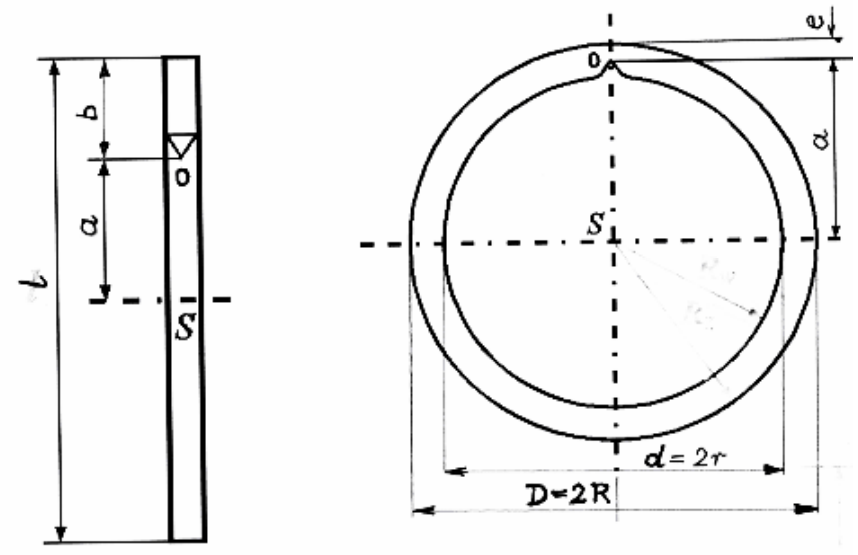
\includegraphics[scale=0.3]{bryly.png}}
\caption{Bryły (pręt i pierścień) użyte w ćwiczeniu}
\label{fig:bryly}
\end{figure}

Pomiary okresu drgań brył wprawionych w ruch wahadłowy o niewielkim wychyleniu zostały dokonane stoperem o dokładności $0,01 \unit{s}$.

\newpage

\section{Wyniki pomiarów}
\subsection{Pomiary masy i długości}
\begin{table}[!htbp]
	\caption{Pomiary masy i długości dla pretu}
	\centering
	\def\arraystretch{1.4}
	\begin{tabular}{@{}rcc@{}}
		\toprule
		\begin{tabular}{@{}c@{}}\end{tabular} &
		\begin{tabular}{@{}c@{}}Wartość  \end{tabular} &
		\begin{tabular}{@{}c@{}}Niepewność \end{tabular}\\
		\midrule
		$m$ [$\unit{g}$]  &  658   &  1    \\
		$l$ [$\unit{mm}$]  &  738   &  1    \\
		$b$ [$\unit{mm}$]  &  99  &  1    \\
		$a$ [$\unit{mm}$]  &  270  &  1    \\
		\bottomrule
	\end{tabular}
\end{table}
\begin{table}[!htbp]
	\caption{Pomiary masy i długości dla pierścienia}
	\centering
	\def\arraystretch{1.4}
	\begin{tabular}{@{}rcc@{}}
		\toprule
		\begin{tabular}{@{}c@{}}\end{tabular} &
		\begin{tabular}{@{}c@{}}Wartość  \end{tabular} &
		\begin{tabular}{@{}c@{}}Niepewność \end{tabular}\\
		\midrule
		$m$ [$\unit{g}$]  &  1360   &  1    \\
		$D_w$ [$\unit{mm}$]  &  249   &  1    \\
		$D_z$ [$\unit{mm}$]  &  279  &  1    \\
		$R_w$ [$\unit{mm}$]  &  124,5  &  1    \\
		$R_z$ [$\unit{mm}$]  &  139,5  &  1    \\
		$e$ [$\unit{mm}$]  &  9,7  &  0,05    \\
		$a$ [$\unit{mm}$]  &  129,8  &  0,05    \\
		\bottomrule
	\end{tabular}
\end{table}




\subsection{Pomiary okresu drgań}
\begin{table}[!htbp]
\caption{Pomiary okresu drgań dla prętu}
\centering
\def\arraystretch{1.4}
\begin{tabular}{@{}rccc@{}}
\toprule
\begin{tabular}{@{}c@{}}Lp.\end{tabular} &
\begin{tabular}{@{}c@{}}Liczba okresów $k$\end{tabular} &
\begin{tabular}{@{}c@{}}Czas $t$ dla $k$ okresów [$\unit{s}$]\end{tabular} &
\begin{tabular}{@{}c@{}}Czas 1 okresu [$\unit{s}$]\end{tabular}\\
\midrule
1  &  30  &  39,72   &    1,324  \\
2  &  30  &  39,61   &    1,320  \\
3  &  30  &  39,58   &    1,319  \\
4  &  30  &  39,66   &    1,322  \\
5  &  30  &  39,48   &    1,316  \\
6  &  30  &  39,60   &    1,320  \\
7  &  30  &  39,46   &    1,315  \\
8  &  30  &  39,33   &    1,311  \\
9  &  50  &  65,68   &    1,314  \\
10 &  50  &  65,75   &    1,315  \\
\midrule
   &  &    Wartość średnia okresu $T$: 1,318&\\
\midrule
   &  &   Niepewność $u(T)$: 0,000015 & \\
\bottomrule
\end{tabular}
\end{table}
\begin{table}[!htbp]
	\caption{Pomiary okresu drgań dla pierścienia}
	\centering
	\def\arraystretch{1.4}
	\begin{tabular}{@{}rccc@{}}
		\\
		\toprule
		\begin{tabular}{@{}c@{}}Lp.\end{tabular} &
		\begin{tabular}{@{}c@{}}Liczba okresów $k$\end{tabular} &
		\begin{tabular}{@{}c@{}}Czas $t$ dla $k$ okresów [$\unit{s}$]\end{tabular} &
		\begin{tabular}{@{}c@{}}Czas 1 okresu [$\unit{s}$]\end{tabular}\\
		\midrule
		1  &  30  &  31,04   &    1,035  \\
		2  &  30  &  30,83   &    1,028  \\
		3  &  30  &  31,01   &    1,034  \\
		4  &  30  &  31,05   &    1,035  \\
		5  &  30  &  31,12   &    1,037  \\
		6  &  30  &  30,96   &    1,032  \\
		7  &  30  &  30,91   &    1,030  \\
		8  &  30  &  31,16   &    1,039  \\
		9  &  30  &  31,17   &    1,039  \\
		10 &  30  &  30,86   &    1,029  \\
		\midrule
		&  &    Wartość średnia okresu $T$: 1,034&\\
		\midrule
		&  &   Niepewność $u(T)$: 0,000014 & \\
		\bottomrule
	\end{tabular}
\end{table}





\newpage

\section{Opracowanie wyników dla pręta}

\subsection{Moment bezwładności $I_0$}

Wartość momentu bezwładności względem osi obrotu $O$:

$$ I_0 = \frac{mgaT^2}{4\pi^2} = 0,07665 \unit{[kg \cdot m^2]} $$

\subsection{Moment bezwładności $I_S$}
Wartość momentu bezwładności względem środka masy:

$$ I_S = I_0 - ma^2 = 0,0287 \unit{[kg \cdot m^2]} $$

\subsection{Moment bezwładności względem osi przechodzącej przez środek masy}

Wartość momentu bezwładności względem osi przechodzącej przez środek masy wyliczona z wartości geometrycznych:

$$ I_S^{(geom)} = \frac{1}{12}ml^2 = 0,02987 \unit{[kg \cdot m^2]}$$

\subsection{Niepewności pomiaru}

Niepewność pomiaru masy (ważonej na wadze o dokładności $1 \unit{g}$):

$$ u(m) = 0,001 \unit{kg} $$

Niepewność pomiaru długości pręta (mieżonego linijką o dokładności $1 \unit{mm}$):

$$ u(l) = 0,001 \unit{m} $$

Niepewność pomiaru odległości $a = l/2 - b$:

$$ u(a) = 0,0005 \unit{m} $$

Niepewność typu A pomiaru okresu $T$:

$$\overline{T}=\frac{\sum{T_i}}{n}=1,318 \unit{[s]}$$
$$u(T)=\sqrt{\frac{\sum{(T_i-\overline{T})^2}}{n(n-1)}} = 0,00000167\unit{[s]}$$

gdzie: $n$ - ilość pomiarów, $\overline{T}$ - średni okres drgań.

\subsection{Niepewność złożona}

Niepewność złożona momentu bezwładności $I_0$:

$$ \frac{u(I_0)}{I_0} = \sqrt{ \left[ \frac{u(m)}{m} \right]^2 + \left[ \frac{u(a)}{a} \right]^2 + \left[ 2 \frac{u(T_0)}{T_0} \right]^2} $$

$$ u(I_0) = 0,000306 \unit{kg \cdot m^2} $$

Niepewność złożona momentu bezwładności $I_S$:

$$ u(I_S) = \sqrt{ \left[ u(I_0) \right]^2 + \left[ a^2 \cdot u(m) \right]^2 + \left[-2 a m \cdot u(m) \right]^2 } $$

$$ u(I_S) = 0,000475 \unit{kg \cdot m^2} $$

Niepewność złożona momentu bezwładności obliczonego geometrycznie $I_S^{(geom)}$:

$$ \frac{u(I_S^{(geom)})}{I_S^{(geom)}} = \sqrt{\left[ \frac{u(m)}{m} \right]^2 + \left[ 2\frac{u(l)}{l} \right]^2 } $$

$$ u(I_S^{(geom)}) = 0,000012 \unit{kg \cdot m^2} $$


\subsection{Sprawdzenie zgodności wyników}
Wyniki nie są zgodne, gdyż wartość:

$$ \frac{ \left| I_S - I_S^{(geom)} \right| }{\sqrt{u^2(I_S) + u^2(I_S^{(geom)})}} = 2,49 $$

jest większa od $k = 2$.

\section{Opracowanie wyników dla pierścienia}

\subsection{Moment bezwładności $I_0$}

Wartość momentu bezwładności względem osi obrotu $O$:

$$ I_0 = \frac{mgaT^2}{4\pi^2} = 0,0469 \unit{[kg \cdot m^2]} $$

\subsection{Moment bezwładności $I_S$}

Wartość momentu bezwładności względem środka masy:

$$ I_S = I_0 - ma^2 = 0,024 \unit{[kg \cdot m^2]} $$

\subsection{Moment bezwładności względem osi przechodzącej przez środek masy}

Wartość momentu bezwładności względem osi przechodzącej przez środek masy wyliczona z wartości geometrycznych:

$$ I_S^{(geom)} = \frac{1}{12}ml^2 = 0,0238 \unit{[kg \cdot m^2]}$$

\subsection{Niepewności pomiaru}

Niepewność pomiaru masy (ważonej na wadze o dokładności $1 \unit{g}$):

$$ u(m) = 0,001 \unit{kg} $$

Niepewność pomiaru promienia $R = \frac{D_z}{2}$ (mierzonego linijką o dokładności $1 \unit{mm}$):

$$ u(R) = 0,0005 \unit{m} $$

Niepewność pomiaru promienia $r = \frac{D_w}{2}$ (mierzonego linijką o dokładności $1 \unit{mm}$):

$$ u(r) = 0,0005 \unit{m} $$

Niepewność pomiaru odległości $a$ (mierzonej suwmiarką o dokładności $0,05 \unit{mm}$):

$$u(a) = 0,000005 \unit{m} $$

Niepewność typu A pomiaru okresu $T$:

$$\overline{T}=\frac{\sum{T_i}}{n}=1,0337 \unit{[s]}$$
$$u(T)=\sqrt{\frac{\sum{(T_i-\overline{T})^2}}{n(n-1)}} = 0,00000016 \unit{[s]}$$

gdzie: $n$ - ilość pomiarów, $\overline{T}$ - średni okres drgań.

\subsection{Niepewność złożona}

Niepewność złożona momentu bezwładności $I_0$:

$$ \frac{u(I_0)}{I_0} = \sqrt{ \left[ \frac{u(m)}{m} \right]^2 + \left[ \frac{u(a)}{a} \right]^2 + \left[ 2 \frac{u(T_0)}{T_0} \right]^2} $$

$$ u(I_0) = 0,0000389 \unit{kg \cdot m^2} $$

Niepewność złożona momentu bezwładności $I_S$:

$$ u(I_S) = \sqrt{ \left[ u(I_0) \right]^2 + \left[ a^2 \cdot u(m) \right]^2 + \left[-2 a m \cdot u(m) \right]^2 } $$

$$ u(I_S) = 0,000356 \unit{kg \cdot m^2} $$


Niepewność złożona momentu bezwładności obliczonego geometrycznie $I_S^{(geom)}$:

$$ u(I_S^{(geom)}) = \sqrt{ \left[ \frac{R^2 + r^2}{2} u(m) \right]^2 + \left[ mRu(R) \right]^2 + \left[ mru(r) \right]^2 } $$


$$ u(I_S^{(geom)}) = 0,000128 \unit{kg \cdot m^2} $$

\subsection{Sprawdzenie zgodności wyników}

Wyniki są zgodne, gdyż wartość:

$$ \frac{ \left| I_S - I_S^{(geom)} \right| }{\sqrt{u^2(I_S) + u^2(I_S^{(geom)})}} = 0,49 $$

jest większa od $k = 2$.


\section{Wnioski}

W przypadku obu brył niepewności momentu bezwładności liczone na podstawie wzorów geometrycznych są mniejsze niż niepewności momentu bezwładności wyznaczanego na podstawie okresu drgań. Wnioskujemy zatem, że metoda ta jest dokładniejsza. W przypadku pierścienia udało nam się przeprowadzić pomiary na tle dokładnie, że wartości są zgodne. Natomiast w przypadku pręta wyniki są poza granicami niepewności rozszerzonej. Być może jest to związane z błędem systematycznym pomiaru okresu $T$ powodowanym przez tłumienie drgań przez ośrodek oraz tarcie na punkcie styku pręta ze statywem.

\end{document}
